
\documentclass[12pt]{amsart}

\usepackage{enumerate,amsmath,amssymb,amsthm}

\usepackage{arydshln}
\usepackage{dashrule}
\usepackage{ulem}
\usepackage{cite}
\usepackage{graphicx}
\graphicspath{ {/Users/alechewitt/Desktop/SULI_paper_images/} }

\newcommand{\comment}[1]{}

\begin{document}
\title{\underline{Introduction, methods, and materials}}
\author{Alec Hewitt}
\maketitle

\setlength\parindent{24pt}

\section{\underline{Introduction and Background}}

\indent The Gaia database has data for over 1 billion stars. This is only roughly 1\% of the stars
contained in the Milky Way but there is still a plethora of data to explore some of the structures
nature can produce. With this amount of data, we cannot rely on traditional programming methods to identify such patterns as this may take an incredibly long time. This is where machine
learning comes in. The main software that will be used is FAISS (Facebook AI Similarity
Search) which is a C++ library but also contains an interface in Python; Python is the language
used in this project. The idea to apply machine learning to astronomical data for this project
came from Maurice Garcia-Sciveres who saw an analogy between particle physics and astro-physics.\\

\indent In particle physics, when particles collide they fly off into particle detectors which detect
the positions of these particles at certain discrete points in space. To know the trajectories they
must “connect the dots” to identify which particles came from where. This is a fairly simple task
to connect the dots for a small number of particles, but once there are thousands of particles,
such tasks become insurmountable. To deal with such a problem, they must figure out a way to
systematically connect the dots. One such method is to take each dot and find the k-nearest
neighbors of that dot, this turns into a combinatorics problem since we are finding every possible
combination of dots and choosing the combinations that correspond to the smallest distances.\\

\indent This can be a computationally intense problem. One way around this is to use a similarity search
that returns the k-nearest neighbors of every particle; such a method requires machine learning.
This project will use a similar technique to analyze data from Gaia eDR3 (2),(3). However, instead of "connecting the dots" of particle trajectories this project provides a tool to connect clusters, where the analogy of a particle in this project is a cluster. Such a tool could be used to locate and map out astronomical objects, such as stellar streams.

\indent It is a trivial task to identify whether stars are similar in position, just look at the regions that are clustered.
While these stars may contain similar properties, this project seeks to find clusters of stars in a
similar but more subtle way. Gaia eDR3 has many useful properties that extend beyond just the
position of the star. Only features within the Gaia database identified as “good” measurements
and features that most stars possess are used. Once a dataset has been obtained, the similarity
search can begin. This search involves using the Python package “FAISS” which stands for
“Facebook AI Similarity Search”.\\

\indent A basic example of how this works is as follows: positions of a group of stars are given
within a dataset, the objective is to find the clusters within this data set, i.e., the regions of the
dataset that are the “clumpiest”. FAISS has a function called “Inverted File Index” or “IVF”. This
function takes in the set of vectors, the number of clusters needed, and the number of data points
desired for each cluster and spits out a list of clusters. This project will use a similar method except it will use higher dimensional vectors, however, this particular example can be useful as the
human eye can identify such clusters and this can be used to ensure the methods are returning
intuitively correct results.\\

\indent The research group consists of Maurice Garcia-Sciveres, Xiangyang Ju, and Alec Hewitt.
Maurice is the mentor of this project, Xiangyang is the associate mentor and Alec is the intern.
The purpose of the research group is to have meetings at least once a week to brainstorm. During
these meetings, the intern discusses what progress has been made, possible issues that were encountered, and what can be improved. The mentor and the associate mentor then evaluate the
progress and determine whether the intern is on the right track or whether his methods and direction need to be modified. The results for that week are evaluated and a list of tasks is created to
complete by the next meeting. The intern takes these tasks and attempts to complete them
promptly and regular updates are given throughout the week.\\

\indent Any details that were not covered in the meeting are expanded upon by the intern by using their best judgment. Questions regarding the tasks of the assignment are generally directed
towards the associate mentor while questions regarding the overall direction of the project are
directed towards the mentor.\\

\comment{
\section{\underline{Methods}}
\section*{Obtaining and Preprocessing the Dataset}
\indent The initial dataset was obtained through the Gaia archive using "ADQL" for the search, (1) contains many helpful examples on how this is done. Here we retrieve all features for stars with parallax$>$33.333333, which corresponds to a distance estimate (reciprocal of parallax) of $<$ 30 pc.\\

\indent Once the dataset was obtained, some measurements are missing and are given by "Nan". For this analysis only features that have measurements for more than 92\% entries are used to identify clusters. Although the positions are not used to identify clusters, they will be used to plot and connect clusters.\\
\indent  The data is further constrained by requiring: \\
\begin{align}
\begin{cases}
	$abs('phot\_g\_mean\_flux\_over\_error')$>3,\\
	$abs('phot\_bp\_mean\_flux\_over\_error')$>3,\\
	$abs('phot\_rp\_mean\_flux\_over\_error')$>3,\\
	$abs('astrometric\_excess\_noise')$<3,\\
\end{cases}
\end{align}
 and 'phot\_proc\_mode'==0. The corresponding positions were transformed from galactic coordinates to cartesian, in the galactic basis. The distributions for the accepted features were obtained and analyzed, to determine how to standardize these quantities. To standardize these quantities something similar to the standard deviation must be defined. The distributions for accepted features were not all gaussian so it was decided to use the fullwidth half max as a substitute for the standard deviation. The standardized quantities were thus determined to be $\frac{d_{ij}-\langle d_j \rangle }{\sigma_j}$, where $d_{ij}$ is the ith entry of the jth feature and sigma is the full width half max for the jth accepted feature.

\section*{Obtaining Clusters}
\indent Before obtaining the clusters a crucial question to ask is what is the most natural number of clusters in the dataset? There are many solutions to this problem and one of them is known as "Silhouette clustering". The silhouette score is a number that represents how well the data is grouped into n clusters and ranges between -1 and 1, a value of 1 means that the data is grouped perfectly into those n clusters, so a higher value represents a better grouping. the data was grouped into clusters for the total number of clusters varying from 2 to 10 and the silhouette score for each grouping was calculated. The value of n corresponding to the highest silhouette score was used to group the data. (it was noticed that a value of n=2 always corresponded to the best number of clusters so this number of clusters was used moving forward)\\

\indent To obtain the clusters of the dataset the python packages "faiss" and "sklearn" (4) were used. faiss's kmeans function was used and trained on the data. The centroids were then extracted where the number of centroids is given by the silhouette method. An inverted index was initialized using the "IndexIVFFlat" function from the faiss package and it was also trained on the data. This function sorts all data into n clusters, the purpose of using kmeans is to obtain the centroids. The data was sorted to the kmeans centroids using a similarity search on the centroids obtained from k-means. The number of neighbors specified was the length of the dataset. The number of neighbors is irrelevant if large enough since the index will not place more stars in the cluster than the cluster contains. The return of this algorithm is a list of clusters, each entry contains indices for all members of that cluster, the entire set is a partition of the original indices.\\

\section*{Identifying significant clusters}
\indent These indices were used to obtain corresponding positions of all stars in the group of clusters. For each cluster, a line of best fit was fitted to the cluster using svd or singular value decomposition. The goodness of fit was determined using the coefficient of determination or $r^2$ value. Recall that the $r^2$ value typically ranges from 0 to 1 with 1 signifies that the data is fitted well by a line. The most significant cluster is defined as the cluster with the highest $r^2$ score.\\

\section*{Obtaining new datasets}
\indent The line of best fit is then used to calculate the intersection points with the dataset boundaries as follows. Suppose the line of best fit is given by\\
\begin{align}
	\vec{r}(t)=\vec{r}_0 + \vec{v}t,
\end{align}
suppose the line intersects the boundaries of the dataset (which is a ball centered at $(0,0,0)$ in position space) at $t_0$, then the line must intersect the sphere at 
\begin{align}
(x,y,z)=(x_0+v_xt,y_0+v_yt,z_0+v_zt)
\end{align}
Suppose the boundary of the dataset is given by 
\begin{align}
x^2+y^2+z^2=r^2
\end{align}
 where r is the radius of the dataset. Inserting $(x,y,z)$ into the equation of the sphere allows us to find $t_0$ and thus the corresponding intersection points $(x,y,z)$.\\
\indent These intersection points are then inverted back into galactic cordinates, i.e., $(x,y,z) \rightarrow (r,l,b)$. These points are used to obtain another dataset. Since there are two $t_0$ values let them be given by $t_{01}>=t_{02}$ and corresponding galactic coordinates of $(r_0,l_{01},b_{01})$ and $(r_0,l_{01},b_{01})$. The two new datasets are obtained through the Gaia archive by using the constraints:
\begin{align}
\begin{cases}
	16.6666<$parallax$<33.333333,\\
	b_{01}-\theta<b<b_{01}+\theta,\\
	l_{01}-\theta<b<b_{01}+\theta
\end{cases}
\end{align}
 for the first dataset and\\
 \begin{align}
 \begin{cases}
	16.6666<$parallax$<33.333333,\\
	b_{02}-\theta<b<b_{02}+\theta,\\
	l_{02}-\theta<b<b_{02}+\theta
\end{cases}
\end{align} 
for the second dataset. $\theta$ is a parameter to be tuned to the dataset until there are roughly 10000 stars These datasets are extracted and the steps "Preprocessing the dataset", and "Obtaining clusters" are repeated (the direction of the project becomes fuzzy at this point).\\

\section*{Following the cluster}
\indent In these new data, lines of best fit are calculated for each cluster. To identify where the original significant cluster (seed) is headed, each of the lines from the new data are compared with the line corresponding to the seed. To extend the original cluster the new clusters must share certain similarities. First, they must be close in feature space and they must be aligned in the same direction in real space. One way to determine whether they are close in feature space is to throw the test cluster into the original dataset and see if it is placed in the original cluster as the seed. To determine whether they are aligned in the same direction, the direction of the lines of best fit can be determined via the dot product. Suppose the seed has line $\vec{r}_0(t)=\vec{b}_0+\vec{v}_0 t$ and the test cluster has line $\vec{r}_1(t)=\vec{b}_1 + \vec{v}_1 t$, then if they are nearly aligned in the same direction then 
$\frac{\vec{v}_0 \cdot \vec{v}_1 }{||\vec{v}_0|| ||\vec{v}_1||} \approx 1$
}



















\section{\underline{Results }}
	The goal of this paper is to develop an algorithm to locate a stellar stream and follow it, storing the stars contained within the stream along the way. The first step is to figure out how to locate the stellar stream. Since a stellar stream contains stars traveling in a similar direction, as a first step we can expect that the proper motion of such stars would be clustered in feature space. A more accurate approach would be to locate clusters in proper motion + radial velocity space, but since the measurement of radial velocity is very rare among Gaia data, this feature must be omitted. 
\section*{Identifying a Stellar Stream}
	This algorithm will eventually partition the galaxy into many datasets and search for clusters in each one so this method needs to be a quick way of determining whether there is a possible stream or not. One method would be to cluster the data with N clusters, using the inverted Faiss index and create a plot of number of stars vs. cluster. If there are any pre-clusters that have an unusually high amount of stars within it, this hints that these stars may belong to a cluster, this constraint is discussed in the results section. 
	\comment{
	More precisely, if there is a cluster that contains more than twice the average number of stars and contains more than 120\% of any other cluster, there is a decent chance this cluster is part of a cluster. 
	To determine whether this is the case, the algorithm takes a small dataset and performs this analysis on it. It is known that there is a stellar stream called GD1 at the location $(x,y,z)=(-1.364193093355583, 1.6145818620596244, 3.204964878766433)$ (kpc) in equatorial coordinates. (https://iopscience.iop.org/article/10.3847/1538-4357/ab0080/pdf). If the proper motion of the stars within this region are plotted, there is a clear cluster located at roughly $(\mu_{\alpha^*},\mu_{\delta}) \approx (0.02,-0.11)$ (mas)(show the proper motion image). }






\comment{
After plotting the number of stars vs. cluster number shown in figure (show plot), there is a clear spike in the number of stars, if the cluster corresponding to that spike is extracted and the proper motion is plotted (show plot), it is clear that this is the correct cluster. This is a quick way to eliminate datasets that have a low chance of containing a stellar stream and saving a more detailed analysis for the datasets that likely contain a stream. 



2 images
}




\comment{
An Important Note on Search Queries
An important note before continuing: within the searching language of the Gaia archive (ADQL) if we requested a cube by the constraints,
\begin{align}
	x_{min}<x<x_{max}\\
	y_{min}<y<y_{max}\\
	z_{min}<z<z_{max}
\end{align},\\
this would take a long time and would likely time out. This is because the search engine is going through every data point in the Gaia catalog and performing calculations to covert spherical coordinates into cartesian. A way to improve the speed of the search would be to first apply constraints on b, and l to drastically cut down the amount of calculations that need to be performed. A good way to do this would be to constrain b and l so that the cube barely fits within these constraints and perhaps 2 corners touch the constraints as shown in figure (?)




Image





Thus, a better query for this stellar stream would be,

\begin{align}
	l_{min}<l<l_{max}\\
	 b_{min}<b<b_{max}\\
	x_{min}<x<x_{max}\\
	y_{min}<y<y_{max}\\
	z_{min}<z<z_{max}.
\end{align}
}





\section*{Automation }
	The next step is to automate this process and a first step is to automate dataset extraction. In order to do this, small datasets are extracted out of the Gaia archive one at a time. To ensure that the same dataset is not analyzed twice an array of points is preselected, each one represents the center of a dataset. This array of points will be referred to as a lattice. The boundaries of the dataset are calculated and they are of the following form
\begin{align}
\ell_0 - \frac{\Delta \ell}{2} < \ell < \ell_0 + \frac{\Delta \ell}{2}\\
b_0 - \frac{\Delta b}{2} < b < b_0 + \frac{\Delta b}{2}\\ 
d_0 - \frac{\Delta d}{2} < d < d_0 + \frac{\Delta d}{2}
\end{align}
where $(\ell_0,b_0,d_0)$ represents the center of the dataset in galactic coordinates. So each lattice point has a parameter set associated with it.
	

 The algorithm takes a random point within the lattice as well as its associated parameter set and removes it from the lattice. It uses the parameter set to plug into the Gaia archive to automatically download, retrieve and store the dataset using the python package "selenium" and the software called “chromedriver”. The program then retrieves this from the file and stores it as a dataframe, it then performs the cluster analysis to determine whether the dataset could contain a stream or not. It then takes the information from this analysis and stores it in an array that is in a one to one correspondence with the array of points. This is the process of finding seeds in order to follow the stream. 

\section*{Following the Stream} 
Once the seeds are found then the algorithm takes all neighboring datasets and analyzes them for stellar streams, if stellar streams are found it keeps searching all boxes around the boxes containing stellar streams until no more stellar streams are found. This has the effect of finding the full cross section of the stream. Then the center of this cross section is determined, a line is fitted to it so that it aims in the direction of the stellar stream and the nearest boxes that it intersects, it analyzes and if it contains a stellar stream, it locates the cross section and keeps repeating this process until the full stellar stream is located.

Once the seeds are found the algorithm will then take all neighboring datasets datasets and analyze each of those datasets for clusters, the neighboring datasets of the original seed is referred to as the first layer. If a cluster is found it appends those points to the list of seeds. For each of these seeds, the algorithm will find the neighboring datasets of each of those seeds that have not already been analyzed, this is referred too as the second layer. It will then analyze each of the datasets from the second layer and store the ones that contain clusters. It will then create the neighboring datasets from the 2nd layer, this is called the third layer and so forth. This process continues until there are no more clusters found. This resulting chain of datasets containing clusters may be a part or a whole stellar stream.





\section{\underline{Results}}
A cluster is considered to be significant if it contains at least twice the average number of stars and contains more than 120\% of stars than any other cluster in that set. The number of clusters in the data is 50 if the number of stars is less than 10000 and 50 clusters per 10000 stars if the number of stars is greater than 10000 (rounded down). To determine whether the algorithm works, we consider a dataset with a known stellar stream. It is known that there is a stellar stream called GD1 at the location $(x,y,z)=(-1.364, 1.614, 3.204)$ (kpc) 
in equatorial coordinates. (https://iopscience.iop.org/article/10.3847/1538-4357/ab0080/pdf). 

\begin{figure}[h]
\centering
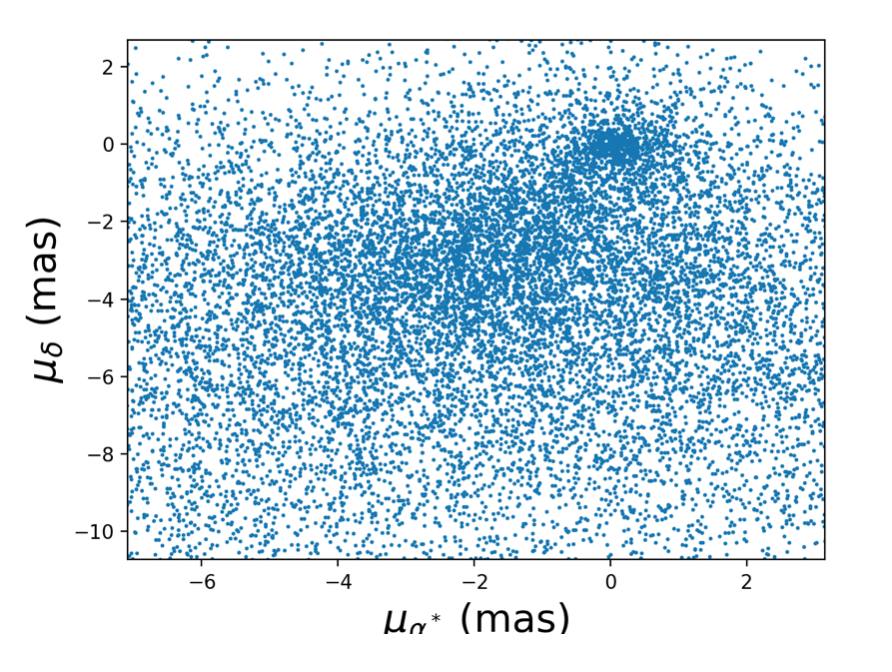
\includegraphics[width=0.5\textwidth]{pm_cluster}
\caption{A plot of proper motion}
\end{figure}


If the proper motion of the stars within this region are plotted, there is a clear cluster located at roughly $(\mu_{\alpha^*},\mu_{\delta}) \approx (0.02,-0.11)$ (mas).




After plotting the number of stars vs. cluster number shown in figure 2, there is a clear spike in the number of stars, if the cluster corresponding to that spike is extracted and the proper motion is plotted (show plot), it is clear that this is the correct cluster; this is evidence that this method works for identifying streams. This method is a quick way to eliminate datasets that have a low chance of containing a stellar stream and saving a more detailed analysis for the datasets that likely contain a stream. 

\begin{figure}[h]
\centering
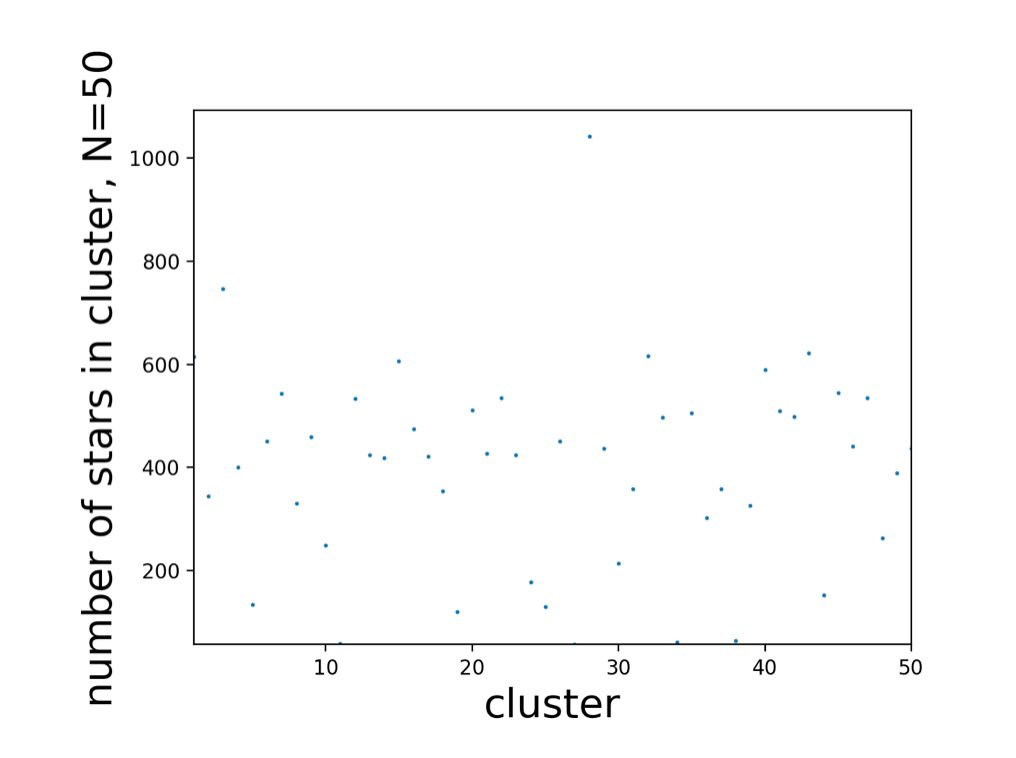
\includegraphics[width=0.5\textwidth]{num_vs_clust}
\caption{A plot showing the number of stars in each cluster on the y axis and the corresponding cluster on the x}
\end{figure}

\begin{figure}[h]
\centering
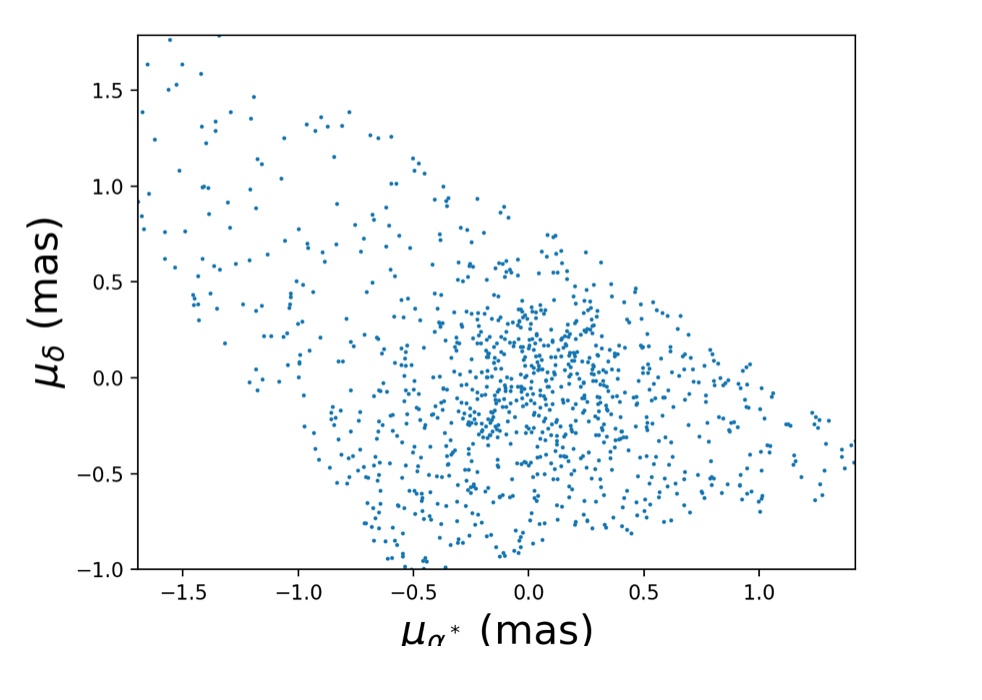
\includegraphics[width=0.5\textwidth]{pm_sig_clust}
\caption{A plot of the significant cluster}
\end{figure}

Now that the method is confirmed to work, the results of the overall algorithm is discussed.
As discussed in the methods section, the algorithm preselects points each representing a dataset. We use a disk that is centered at the sun and parallel to the galactic plane. This disk has a radius of roughly 35 kpc is composed of a lattice of each point. We exclude distances that are less than 2 kpc

\begin{figure}[h]
\centering
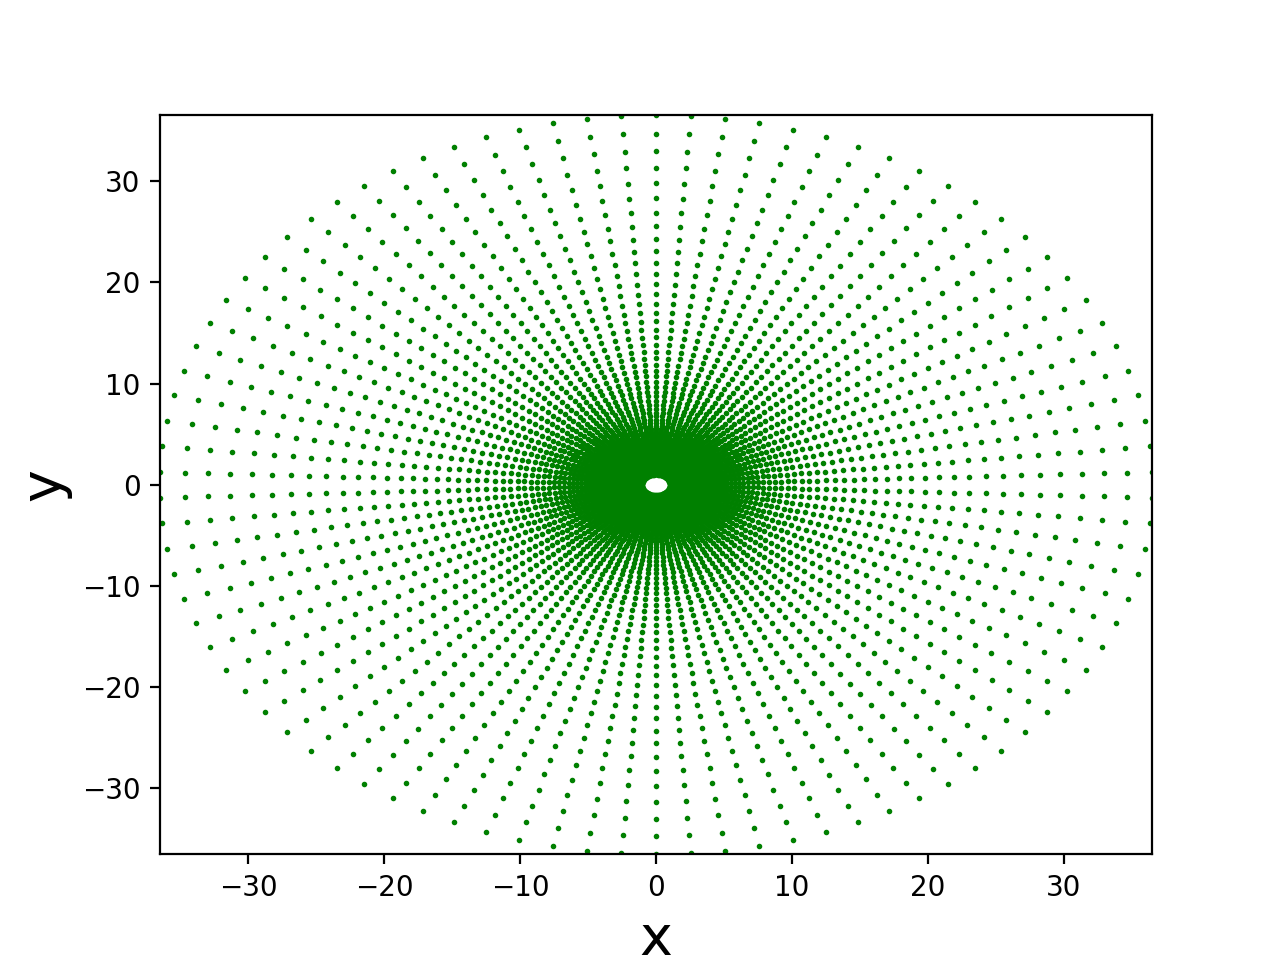
\includegraphics[width=0.5\textwidth]{plane_lattice}
\caption{A lattice of points centered around the sun, each point represents a dataset}
\end{figure}

A typical dataset looks like a sector of a sphere and resembles a cube shown below.

\begin{figure}[h]
\centering
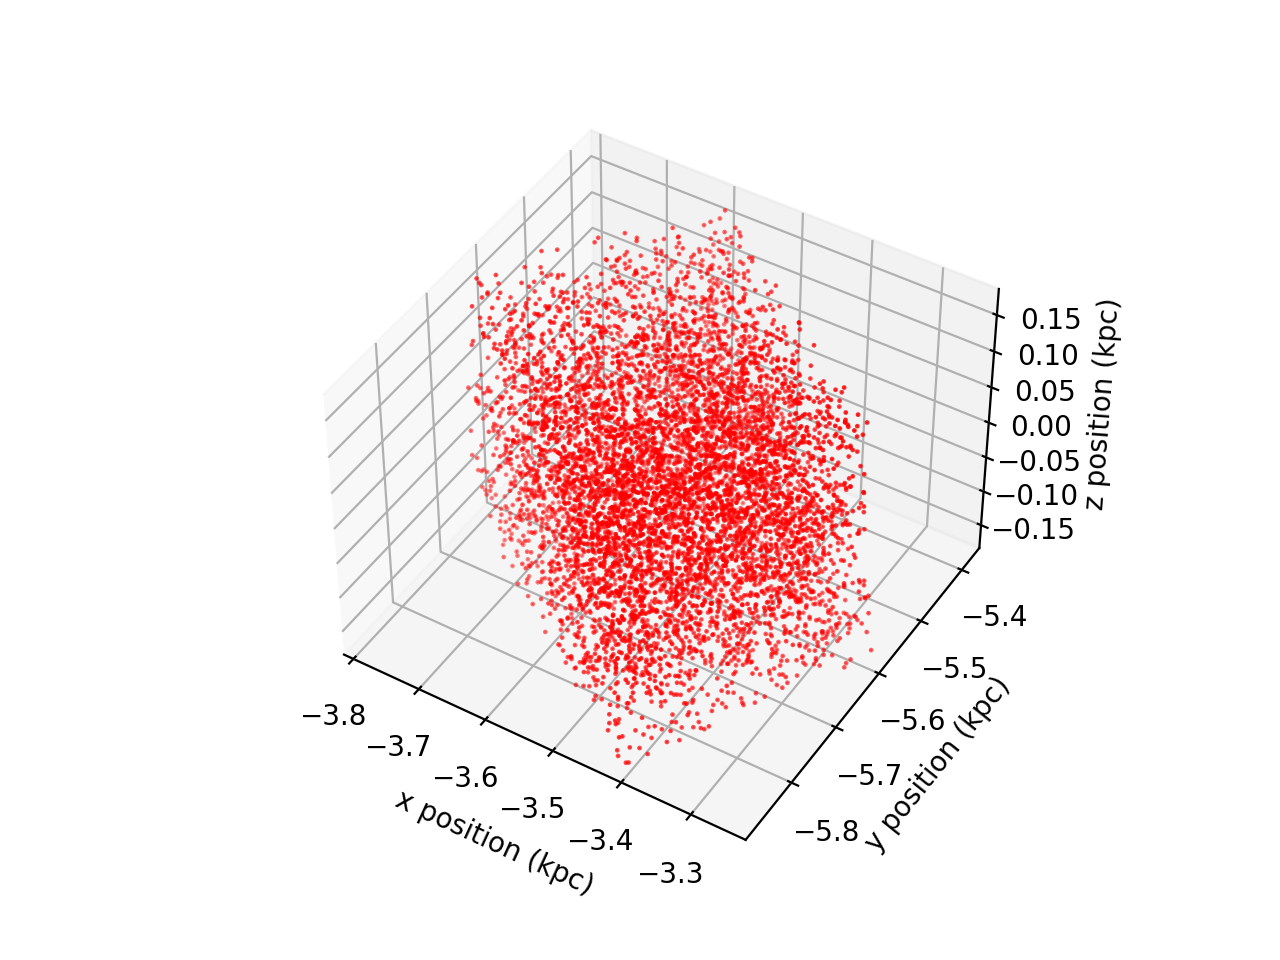
\includegraphics[width=0.5\textwidth]{data_set_2d}
\caption{A typical dataset}
\end{figure}

The bounds of the dataset are discussed in the methods section. Here we take $\Delta b = 3^{\circ}$ and $\Delta l = 4^{\circ}$. The radial thickness has the property that it equals the arc-length of $b$. That is $\Delta d_i = d_{i-1} \Delta b$, where $\Delta b$ is given in radians and $d_i=d_{i-1} + \Delta d_{i-1}$. \\
The algorithm scans each of the lattice points one by one for significant clusters. If a significant cluster is found, the algorithm checks all nearest neighbors for stellar streams. To search out of the plane the lattice must be extended into 3-D as a spherical lattice shown below.

\begin{figure}[h]
\centering
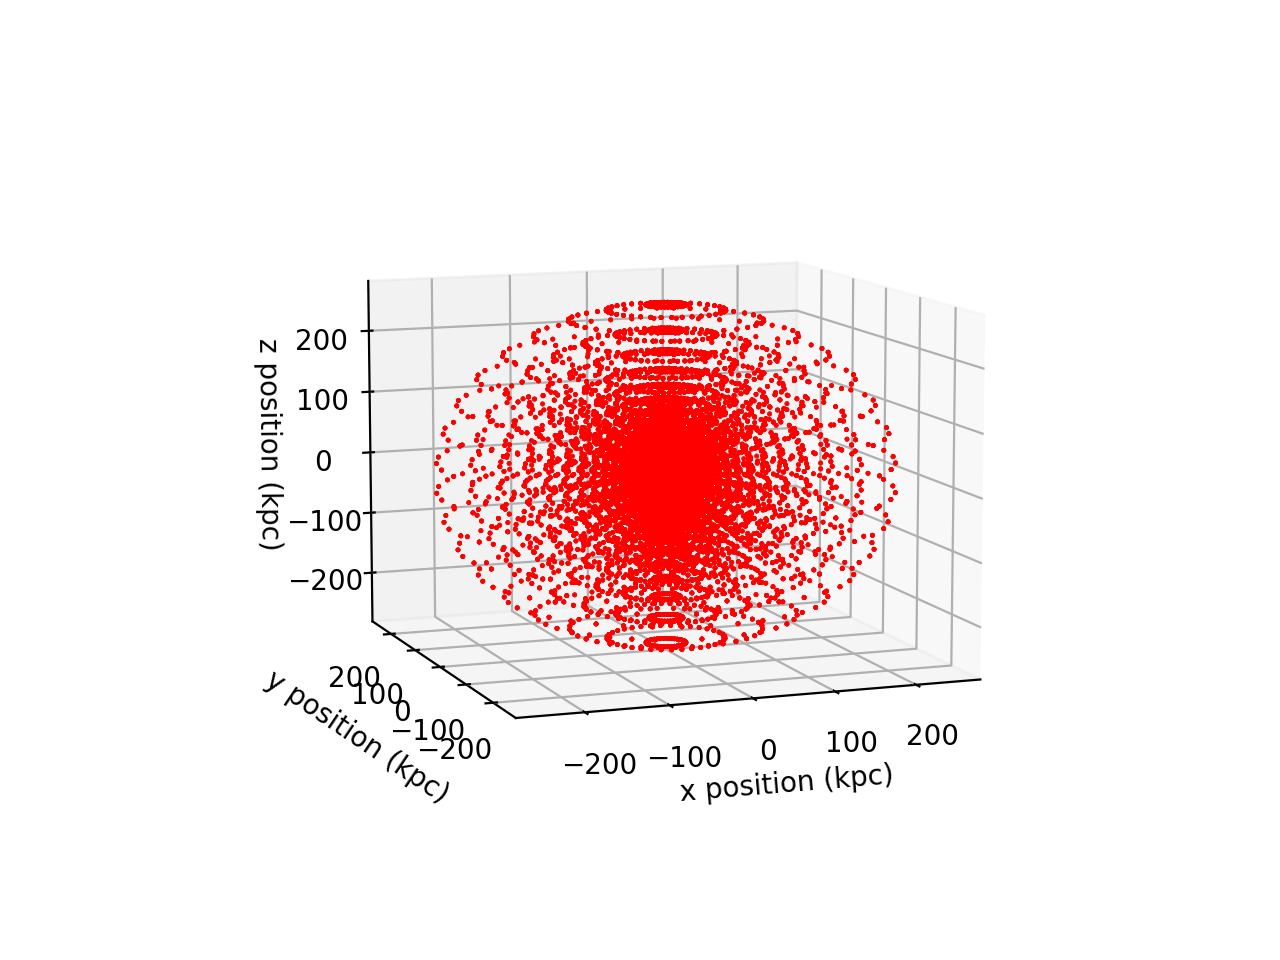
\includegraphics[width=0.5\textwidth]{spherical_lattice}
\caption{A spherical lattice}
\end{figure}

Once a cluster is found, the algorithm searches all nearest neighbors shown in the below image

\begin{figure}[h]
\centering
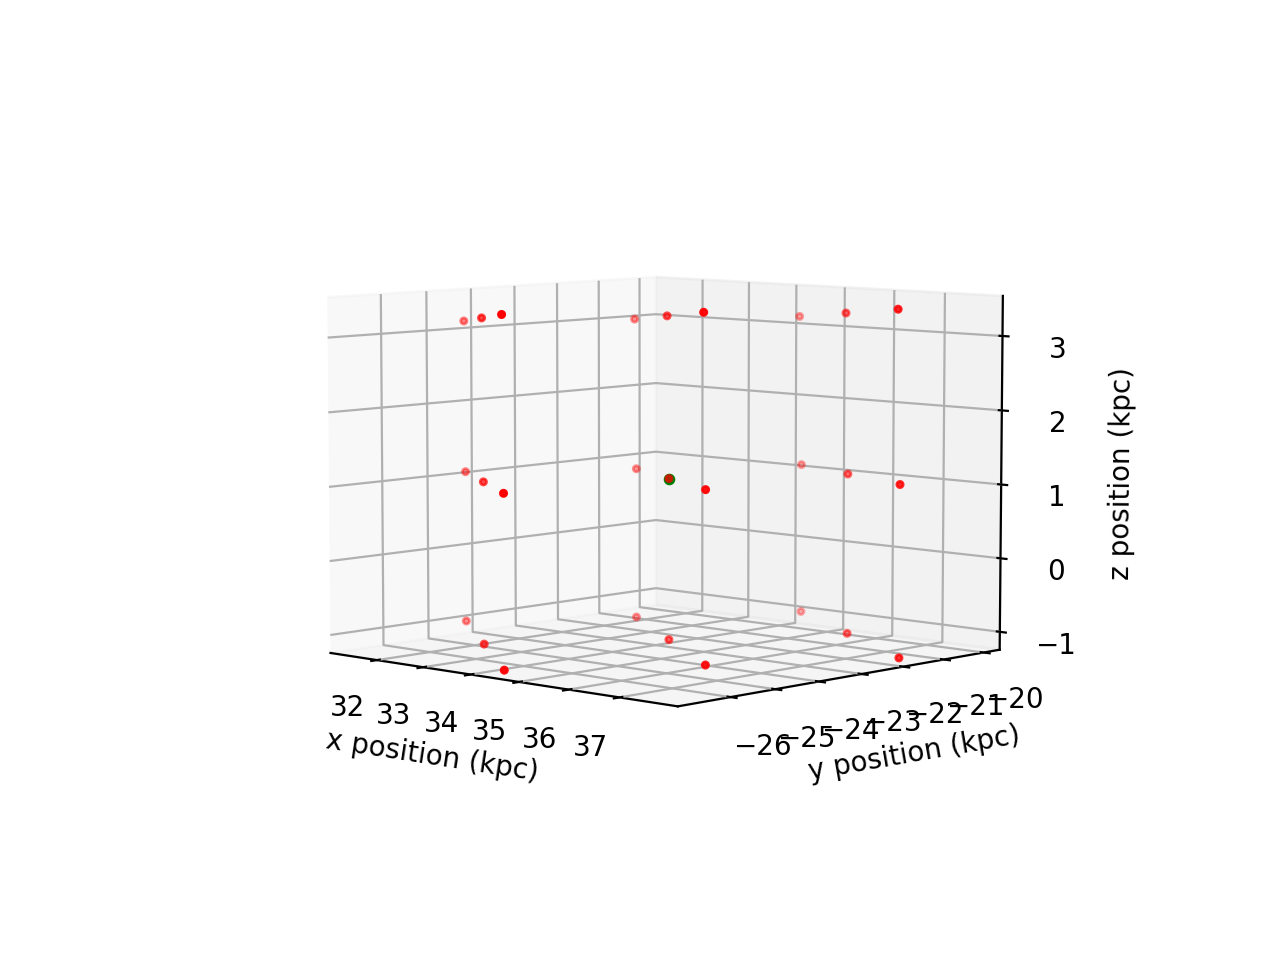
\includegraphics[width=0.5\textwidth]{search_around}
\caption{Neighboring set of a significant dataset, the dark point contains a significant cluster}
\end{figure}

If a neighbor contains a significant cluster, this process is repeated as discussed previously.


\section{\underline{Discussion}}
\indent The methods discussed provide a promising tool to locate and track clusters. When a cluster is present the plots of “number of stars vs. clusters” illustrate a clear peak, this peak corresponds to a cluster. When there is no cluster present there is no longer a peak that sticks out clearly and the algorithm will indicate this. \\
\indent The algorithm designed to scan the galactic plane must scan thousands of datasets, each dataset can take several minutes. Furthermore, when a seed for the cluster is found, tracking the cluster involves scanning 26 datasets around the dataset containing the cluster and for each of those it scans all neighboring datasets that have not been previously analyzed. This process can be very time consuming as well. An obvious improvement to this algorithm would be to incorporate multiprocessing. This would allow the algorithm that scans the galactic plane to become increasingly fast, depending on how many cores the machine possesses. The algorithm that tracks can be made much faster as well  since instead of scanning all neighboring datasets one by one, each neighboring dataset can be given to a separate core and scan of each layer could equal the same amount of time as just scanning a single dataset.\\
\indent This program works for larger radii, currently it works best for distances exceeding 2 kpc from the sun. This was an unexpected difficulty. Datasets that are close to the sun all possess clusters. These clusters are centered at (0,0) which suggests they are traveling in the same direction as the sun. A possible reason for this tight cluster is due to the distance from the sun. For small distances it can be common for the angular velocity to exceed 100 mas/yr whereas for larger distances large angular velocities become exceedingly rare. A solution would be to exclude clusters whose centers are close to (0,0).
	
	


\section*{References}
\begin{enumerate}
\item https://gea.esac.esa.int/archive-help/adql/examples/index.html\\
\item Gaia Collaboration et al. (2016b): The Gaia mission (provides a description of the Gaia mission including spacecraft, instruments, survey and measurement principles, and operations);
\item Gaia Collaboration et al. (2020b): Gaia EDR3: Summary of the contents and survey properties.
\item @article{scikit-learn,
 title={Scikit-learn: Machine Learning in {P}ython},
 author={Pedregosa, F. and Varoquaux, G. and Gramfort, A. and Michel, V.
         and Thirion, B. and Grisel, O. and Blondel, M. and Prettenhofer, P.
         and Weiss, R. and Dubourg, V. and Vanderplas, J. and Passos, A. and
         Cournapeau, D. and Brucher, M. and Perrot, M. and Duchesnay, E.},
 journal={Journal of Machine Learning Research},
 volume={12},
 pages={2825--2830},
 year={2011}
}
\end{enumerate}






\end{document}
